\section{Darstellung}

\begin{defi}{Darstellung (ISO/OSI)}
    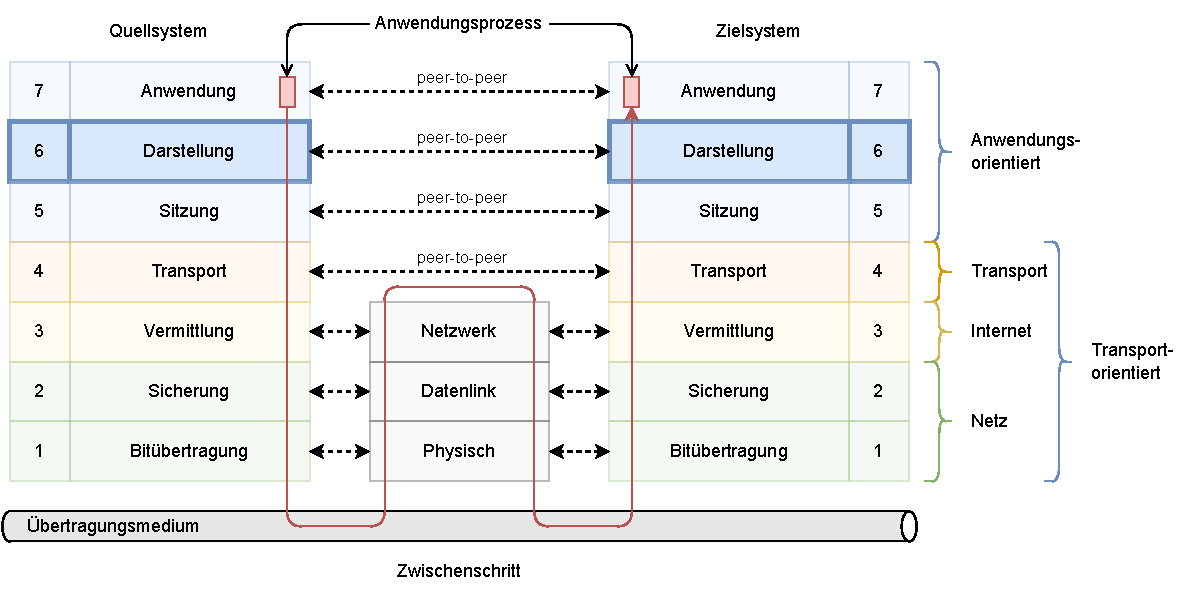
\includegraphics[width=\textwidth]{includes/figures/defi_iso_osi_presentation.pdf}
\end{defi}

\begin{bonus}{Probleme bei der Datenübertragung}
    \begin{itemize}
        \item Heterogenität in verteilten System:

              \begin{itemize}
                  \item Plattformen (Betriebssystem, Hardware)
                  \item Programmiersprachen, APIs
              \end{itemize}
        \item Heterogene Hardware-Architekturen:

              \begin{itemize}
                  \item Zeichencodierung (ASCII, UTF8)
                  \item Reihenfolge der internen Speicherung von Bytes
              \end{itemize}
    \end{itemize}
\end{bonus}

\begin{example}{Little-Endian / Big-Endian}
    Dieses Problem betrifft Datentypen, die aus mehreren Byte zusammengesetzt sind.

    32 Bit-Ganzzahlen benötigen 4 Byte Speicherplatz\footnote{Hier betrachten wir beispielsweise den Typ \emph{uint}}:

    \begin{center}
        \begin{tabular}{|cc|cc|cc|cc|}
            \multicolumn{2}{c}{\textbf{MSB}}   & \multicolumn{4}{c}{}               & \multicolumn{2}{c}{\textbf{LSB}}                                                                             \\\hline
            \multicolumn{2}{|c}{\texttt{0xA0}} & \multicolumn{2}{|c}{\texttt{0xB0}} & \multicolumn{2}{|c}{\texttt{0xC0}} & \multicolumn{2}{|c|}{\texttt{0xD0}}                                     \\\hline
            $16^7$                             & $16^6$                             & $16^5$                             & $16^4$                              & $16^3$ & $16^2$ & $16^1$ & $16^0$ \\\hline
        \end{tabular}
    \end{center}

    Als Ausgangswert steht das \emph{höchswertige Byte} (\enquote{most significant byte} bzw. MSB) ($16^7 + 16^6$) am Anfang und das \emph{kleinstwertige Byte} (\enquote{least significant byte} bzw. LSB) ($16^1 + 16^0$) am Ende.

    Big-Endian speichert die Bytes in der Reihenfolge, in der sie im Ausgangswert vorliegen:\\
    \texttt{0xA0}, \texttt{0xB0}, \texttt{0xC0}, \texttt{0xD0}

    Little-Endian speichert die Bytes in der umgekehrten Reihenfolge:\\
    \texttt{0xD0}, \texttt{0xC0}, \texttt{0xB0}, \texttt{0xA0}
\end{example}

\begin{example}{Übertragung von Datenstrukturen}
    Häufig müssen nicht nur Werte, sondern ganze Datenstrukturen übertragen werden.

    \begin{lstlisting}[language=java]
        class Pokemon {
            uint nummer;
            String name;
        }

        Pokemon p = new Pokemon(4, "Glumanda");
        send(p);
    \end{lstlisting}

    Um dieses Objekt zu übertragen muss man die Werte in Bytes umwandeln.

    \begin{center}
        \begin{tabular}{|c|c|c|c|c|c|c|c|c|c|c|c|c|c|c|c|c|c|c|c|}
            \hline
            \multicolumn{4}{|c}{Nummer}     & \multicolumn{16}{|c|}{Name}                                                                                      \\\hline
            \multicolumn{4}{|c}{\texttt{4}} & \multicolumn{16}{|c|}{\texttt{Glumanda}}                                                                         \\\hline
            0                               & 0                                        & 0 & 4 & 4 & 7 & 6 & C & 7 & 5 & 6 & D & 6 & 1 & 6 & E & 6 & 4 & 6 & 1 \\\hline
        \end{tabular}
    \end{center}

    Der übertragene Bitstream sieht demnach wie folgt aus:

    \begin{center}
        \texttt{0000 0000 [...] 0000 0100 | 0100 0111 [...] 0110 0001}
    \end{center}

    Unser Zielsystem weiß, dass ein Pokemon empfangen werden soll.
    Jedoch sieht die Struktur eventuell auf diesem System wie folgt aus:

    \begin{lstlisting}[language=java]
        class Pokemon {
            String name;
            uint nummer;
        }

        Pokemon p = receive();
    \end{lstlisting}

    Demnach teilt dieses System die empfangenen Bytes wie folgt auf:

    \begin{center}
        \begin{tabular}{|c|c|c|c|c|c|c|c|c|c|c|c|c|c|c|c|c|c|c|c|}
            \hline
            0                          & 0                            & 0 & 4 & 4 & 7 & 6 & C & 7 & 5 & 6 & D & 6 & 1 & 6 & E & 6 & 4 & 6 & 1 \\\hline
            \multicolumn{16}{|c}{Name} & \multicolumn{4}{|c|}{Nummer}                                                                         \\\hline
        \end{tabular}
    \end{center}

    Das Pokemon \texttt{NULEOTGluman} mit der Nummer \texttt{25697} wurde somit empfangen.

    Die potentiell entstehenden Probleme lassen sich in zwei Kategorien einteilen:

    \begin{itemize}
        \item Übertragung der grundsätzlichen Struktur der Daten (Serialisierung, Deserialisierung)
        \item Übertragung des konkreten Datenstroms mit einer vereinbarten Kodierung (Marshalling)
    \end{itemize}
\end{example}

\begin{bonus}{Eigenständige Darstellung}
    Wir gehen mit folgender Idee an unser Problem:

    \begin{itemize}
        \item Definiere eine Menge abstrakter Datentypen und eine Kodierung für jeden dieser Typen.
        \item Stelle Werkzeuge zu Verfügung, welche die Datentypen der verwendeten Programmiersprache in die abstrakten Typen übersetzt.
        \item Wenn ein bestimmter Datentyp übertragen werden soll, rufe die Kodierfunktion auf, und übertrage das Ergebnis (Marshalling).
        \item Dekodiere den bit-String und erzeuge eine neue lokale Repräsentation des empfangenen Typs (Unmarshalling).
    \end{itemize}
\end{bonus}

\begin{example}{Datendarstellungsstandards}
    \begin{itemize}
        \item ISO:

              \begin{itemize}
                  \item \texttt{ASN.1} (Abstract Syntax Notation)
              \end{itemize}
        \item Sun ONC-RPC (Open Network Computing):

              \begin{itemize}
                  \item \texttt{XDR} (eXternal Data Representation)
              \end{itemize}
        \item OSF-RPC (Open System Foundation):

              \begin{itemize}
                  \item \texttt{IDL} (Interface Definition Language)
              \end{itemize}
        \item Corba:

              \begin{itemize}
                  \item \texttt{IDL} und \texttt{CDR} (Common Data Representation)
                  \item \texttt{CDR} bildet IDL-Datentypen in Bytefolge ab
              \end{itemize}
        \item W3C:

              \begin{itemize}
                  \item \texttt{XML/SOAP}
                  \item Darstellung aller Datentypen als (Maschinen-)lesbarer Text.
                  \item Zu klären: Zeichencodierung
              \end{itemize}
        \item Java:

              \begin{itemize}
                  \item \texttt{Objektserialisierung}, d.h. Abflachung von Objekten zu einem seriellen Format inkl. Informationen über die Klassen.
                        Deserialisierung ist die Wiederherstellung eines Objektes ohne Vorwissen über die Typen der Objekte.
              \end{itemize}
        \item JavaScript:

              \begin{itemize}
                  \item \texttt{JSON} (JavaScript Object Notation)
              \end{itemize}
    \end{itemize}
\end{example}

\subsection{ASN.1 (Abstract Syntax Notation)}

\begin{defi}{ASN.1 (Abstract Syntax Notation)}
    \emph{ASN.1} ist eine von der ISO genormte Beschreibungssprache zu darstellungsunabhängige Spezifikationen von Datentypen und Werten.
    Diese Notation findet z.B. zur Definition von Managementobjekten bei SNMP Verwendung.

    Elementare Datentypen:\\
    \texttt{Boolean}, \texttt{Integer}, \texttt{Bitstring}, \texttt{Octetstring}, \texttt{IA5String}, \ldots

    Strukturelle Datentypen:

    \begin{itemize}
        \item \texttt{Sequence}: Geordnete Liste von Datentypen (struct in C)
        \item \texttt{Set}: Ungeordnete Menge an Datentypen
        \item \texttt{Sequence OF}: Geordnete Liste von Datentypen des gleichen Datentyps (Array in C)
        \item \texttt{Set OF}: Ungeordnete Menge des gleichen Datentyps
        \item \texttt{Choice}: Ungeordnete Menge von Datentypen, aus der eine Datentypen ausgewählt werden können (Union in C)
    \end{itemize}
\end{defi}

\begin{example}{ASN.1 (Abstract Syntax Notation)}
    % [language=asn.1]
    \begin{lstlisting}
        Pokemon ::= Sequence {
            Nummer Integer,
            Name IA5String
        }
    \end{lstlisting}
\end{example}

\begin{defi}{ASN.1 Übertragungssyntax}
    Zusätzlich zur Bereitstellung einer Datenbeschreibungssprache bietet ASN.1 auch sogenannte \emph{Basic Encoding Rules}, die spezifizieren, wie ASN.1-Objekte über das Netzwerk versendet werden sollten an.

    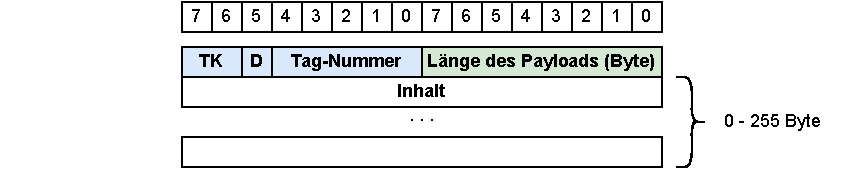
\includegraphics[width=\textwidth]{includes/figures/defi_asn1.pdf}

    \begin{itemize}
        \item Bezeichner: 8 bit

              \begin{itemize}
                  \item Typklasse (TK): 2 bit

                        \begin{tabular}{T|l}
                            00 & Universal        \\
                            01 & Application      \\
                            10 & Context Specific \\
                            11 & Private
                        \end{tabular}
                  \item Datentyp (D): 1 bit

                        \begin{tabular}{T|l}
                            00 & Einfach      \\
                            01 & Strukturiert
                        \end{tabular}
                  \item Tag-Nummer: 8 bit

                        \begin{tabular}{T|l}
                            0000 0000 & End-of-Content (EOC)  \\
                            0000 0001 & Boolean               \\
                            0000 0010 & Integer               \\
                            \multicolumn{2}{c}{\ldots}        \\
                            0001 0000 & Sequence, Sequence OF \\
                            0001 0001 & Set, Set OF           \\
                            \multicolumn{2}{c}{\ldots}        \\
                            0001 0110 & IA5String             \\
                            \multicolumn{2}{c}{\ldots}        \\
                        \end{tabular}
              \end{itemize}
        \item Länge: 8 bit
        \item Wert: 0 - 255 Byte
    \end{itemize}
\end{defi}

\begin{example}{ASN.1 (Abstract Syntax Notation)}
    Fassen wir nun einmal unsere Beispiele zusammen erhalten wir:

    \begin{lstlisting}[language=java]
        class Pokemon {
            uint nummer;
            String name;
        }

        Pokemon p = new Pokemon(4, "Glumanda");
    \end{lstlisting}

    Bzw. in ASN.1:

    % [language=asn.1]
    \begin{lstlisting}
        Pokemon ::= Sequence {
            Nummer Integer,
            Name IA5String
        }
    \end{lstlisting}

    Nun bauen wir den zu übertragenden Bitstream von innen nach außen auf:

    \begin{enumerate}
        \item \texttt{Nummer} ist ein \emph{universaler einfacher Integer}.

              Demnach lautet der Header für \texttt{Nummer}: \texttt{00 0 00010}
        \item \texttt{Name} ist ein \emph{universaler einfacher IA5String}.

              Demnach lautet der Header für \texttt{Name}: \texttt{00 0 10110}
        \item Nun füllen wir den Payload mit den Werten \texttt{4} bzw. \texttt{Glumanda}.
        \item Daraus erhalten wir die benötigte Länge von 4 Byte für \texttt{Nummer} bzw. 16 Byte für \texttt{Name}.
        \item Unser gesamtes Objekt ist eine \emph{universale strukturierte Sequence}.

              Demnach lautet der Header für das \texttt{Pokemon}: \texttt{00 1 10000}
        \item Die Gesamtlänge erhalten wir aus der Summe aller Teilobjekte inkl. Header (in Byte).

              $4 \ \text{(Nummer)} \ + 16 \ \text{(Name)} \ + 2 \cdot 2 \ \text{(Header)} \ = 14_{10} \to 10110_2$
    \end{enumerate}

    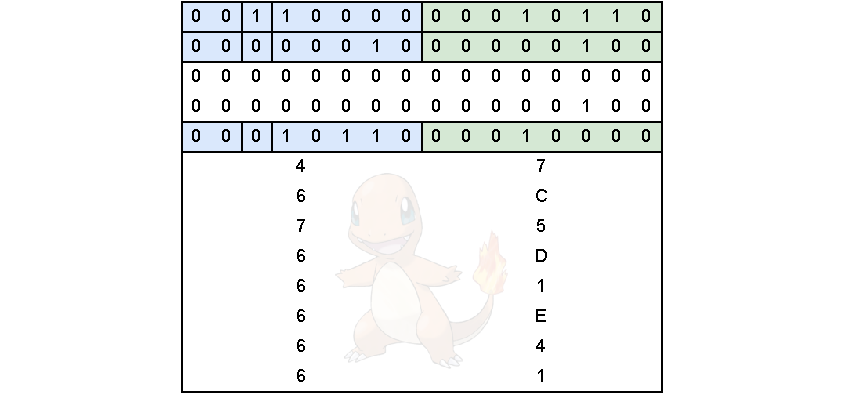
\includegraphics[width=\textwidth]{includes/figures/example_asn1.pdf}
\end{example}

\subsection{XML (eXtensible Markup Language)}

\begin{bonus}{HTML ungeeignet}
    HTML wurde zur Darstellung von Informationen für Menschen und nicht für die Informationesverarbeitung in Programmen entwickelt.

    Die Auszeichnungselemente sind fest vorgegeben und Sind daher nicht zur Beschreibung beliebiger Daten geeignet
    Zusätzlich enthält HTML eine problematische Vermengung von Auszeichnungen und Präsentationssemantik.

    Aus diesen Gründen sollte eine offene, textbasierte Auszeichnungsspache entwickelt werden.
\end{bonus}

\begin{defi}{XML (eXtensible Markup Language)}
    XML ist eine Metasprache zur Strukturierung von Dokumenten und Daten.

    Basis von XML sind beliebige Auszeichnungselemente, die geringen syntaktischen Regeln zu folgen haben.

    XML ist erst wirklich sinnvoll, wenn es in einer Anwendung konkretisiert wird.
    Anwendungen ergeben sich aus:

    \begin{itemize}
        \item \textbf{Namensräumen}:

              Festlegen der semantischen logischen Bedeutung bei Homonymen in den Auszeichnungselementen.
        \item \textbf{Stylesheets}:

              Definition des Erscheinungsbildes von Auszeichnungselementen.
        \item \textbf{Schemata}:

              Beschreiben der Dokumentenstruktur eines bestimmten Typs
    \end{itemize}

    XML-Dokumente enthalten Daten und Sturkturinformationen über die Daten in einem Dokument (\emph{selbstbeschreibend}) und haben feste Strukturvorgaben (\emph{wohlgeformt}).
    Informationen in XML-Dokumenten haben einen Datentyp (\emph{typisiert})

    Jedes Dokument entspricht einer Baumstruktur und haben immer ausschließlich eine Wurzel.

    Für XML-Dokumente gelten folgende Syntaxregeln:

    \begin{itemize}
        \item Jeder Starttag muss einen Endtag haben

              \begin{lstlisting}
<pokemon> ... </pokemon>
<pokemon />
\end{lstlisting}
        \item Verschachtlung nur mit vollständigen Tags möglich.

              \begin{lstlisting}
<pokemon> <name> Glumanda </name> </pokemon> <!-- OK -->
<pokemon> <name> Glumanda </pokemon> </name>  <!-- NOT OK -->
\end{lstlisting}
    \end{itemize}
\end{defi}

\begin{example}{XML (eXtensible Markup Language)}
    % [language=xml]
    \begin{lstlisting}
        <?xml version="1.0" encoding="UTF-8"?>
        <pokemon nummer="4">
            <!-- Glumanda ist besser als Bisasam -->
            <name>Glumanda</name>
        </pokemon>
    \end{lstlisting}
\end{example}

\begin{bonus}{XML Namespace}
    Elementarbezeichner haben ähnlich wie Variablen in Programmiersprachen einen Namensraum.
    Dieser dient der Trennung der Bedeutung der Bezeichner und ermöglicht Inhalte eindeutig zu referenzieren.

    Ein Namespace ist weltweit eindeutig durch eine URI (Uniform Resource Identifier) identifiziert und wird über einen Präfix zugänglich gemacht.
\end{bonus}

\begin{example}{XML Namespace}
    % [language=xml]
    \begin{lstlisting}
        <pokemon nummer="4" xmlns:typ="https://kosy.paddel.xyz/pokemontyp">
            <name>Glumanda</name>
            <typ:primaertyp>Feuer</typ:primaertyp>
            <typ:sekundaertyp />
        </pokemon>
    \end{lstlisting}
\end{example}

\begin{defi}{XML Schemata}
    Ein XML-Schema ist eine XML-Anwendung, mit der die Struktur einer Klasse von XML-Dokumenten beschrieben werden kann.
    Dieses Schema enthält in XML notierte Regeln, die erlaubte Elementarbezeichner, Reihenfolgen, Inhalte und Attribute mit Wertebereichen aufzählen.
    Hierzu existieren vielfältige vordefinierte Datentypen, die Möglichkeiten zur Definition eigener Datentypen und zur Darstellung komplexer Integritätsbedingungen schaffen.
\end{defi}

\begin{example}{XML Schemata (primitive Datentypen)}
    Um primitive Datentypen zu nutzen, kann man sie wie folgt referenzieren:

    % [language=xml]
    \begin{lstlisting}
        <!-- Schema -->
        <xs:element name="pokemonNummer" type="xs:integer" />
    \end{lstlisting}

    Alternativ kann man von primitiven Datentypen erben, um diese um weitere Eigenschaften zu erweitern:

    % [language=xml]
    \begin{lstlisting}
        <!-- Schema -->
        <xs:simpleType name="pokemonNummer" base="xs:integer">
            <xs:minInclusive value="1" />
            <xs:minInclusive value="905" />
        </xs:simpleType>
    \end{lstlisting}

    Diesen Typ können wir nun nutzen, jedoch zusätzlich den eigentlichen primitiven Datentypen dahinter jederzeit austauschen:

    % [language=xml]
    \begin{lstlisting}
        <!-- Dokument -->
        <pokemonNummer>4</pokemonNummer>
    \end{lstlisting}
\end{example}

\begin{example}{XML Schemata (Elementdeklaration)}
    Um einfache Typen mit Attributen vorzugeben, deklariert man ein Element wie folgt:

    % [language=xml]
    \begin{lstlisting}
        <!-- Schema -->
        <xs:element name="pokemon" type="pokemonTyp" />

        <xs:complexType name="pokemonTyp">
            <xs:attribute name="nummer" type="pokemonNummer" />
        </xs:complexType>
    \end{lstlisting}

    Nun können wir bereits erste Pokemon anlegen:

    % [language=xml]
    \begin{lstlisting}
        <!-- Dokument -->
        <pokemon nummer="4" />
    \end{lstlisting}
\end{example}

\begin{example}{XML Schemata (Komplexe Typen)}
    Da wir für unser vollwertiges Pokemon noch einen Namen brauchen, müssen wir unserem erstellten Pokemon weiter Kinderobjekte hinzufügen:

    % [language=xml]
    \begin{lstlisting}
        <!-- Schema -->
        <xs:element name="pokemon" type="pokemonTyp" />

        <xs:complexType name="pokemonTyp">
            <xs:attribute name="nummer" type="pokemonNummer" />
            <xs:sequence>
                <xs:element name="name" type="xs:string" />
            </xs:sequence>
        </xs:complexType>
    \end{lstlisting}

    Jetzt ist unser anfänglich erstelltes Pokemon komplett typisiert:

    % [language=xml]
    \begin{lstlisting}
        <!-- Dokument -->
        <pokemon nummer="4">
            <name>Glumanda</name>
        </pokemon>
    \end{lstlisting}
\end{example}

\begin{bonus}{XML Schemata (Werkzeuge zur Bindung komplexer Typen)}
    Attribute eines komplexen Typs kann man wie folgt angeben:

    \begin{itemize}
        \item \texttt{xs:sequence}:

              Die Inhalte müssen in exakt der Reihenfolge erscheinen, in der sie angegeben werden.
        \item \texttt{xs:all}

              Die Inhalte dürfen in beliebiger Reihenfolge angegeben werden.
              Jedes Element muss dabei exakt einmal instanziiert werden.
              Das hinzufügen weiterer Elemente, die nicht angegeben wurden, ist nicht erlaubt.
        \item \texttt{xs:choice}

              Von den aufgeführten Inhalten muss genau ein frei wählbares instanziiert werden.
    \end{itemize}

    Diese Kompositoren können um weitere Tags ergänzt werden.

    \begin{itemize}
        \item \texttt{minOccurs} gibt an wie oft ein Element mindestens erscheinen muss
        \item \texttt{maxOccurs} gibt an wie oft ein Element maximal erscheinen darf
        \item \texttt{default} gibt den Wert eines Elements an, wenn es vorhanden jedoch leer ist.
    \end{itemize}
\end{bonus}

\begin{bonus}{Abgeleitete Typen}
    Durch abgeleitete Typen wird die Basis eingeschränkt oder erweitert.

    Mögliche Tags sind:

    \begin{itemize}
        \item \texttt{restriction}: Einschränkung des Wertebereichs
        \item \texttt{list}: Auflistung verschiedener Werte
        \item \texttt{union}: Vereinigung mehrerer Typen
        \item \texttt{extension}: Erweiterung in einen komplexen Typen
    \end{itemize}
\end{bonus}

\begin{example}{XML Schemata}
    Fassen wir nun einmal alle Beispiele zusammen und ergänzen Team:

    % [language=xml]
    \begin{lstlisting}
        <!-- Schema -->
        <xs:element name="pokemon" type="pokemonTyp" />
        <xs:element name="team" type="teamTyp" />

        <xs:simpleType name="pokemonNummer" base="xs:integer">
            <xs:minInclusive value="1" />
            <xs:minInclusive value="905" />
        </xs:simpleType>

        <xs:complexType name="pokemonTyp" xmlns:typ="https://kosy.paddel.xyz/pokemontyp">
            <xs:attribute name="nummer" type="pokemonNummer" />
            <xs:sequence>
                <xs:element name="name" type="xs:string" />
                <xs:element name="primaertyp" type="typ" default="Normal" />
                <xs:element name="sekundaertyp" type="typ" minOccurs="0" />
            </xs:sequence>
        </xs:complexType>

        <xs:complexType name="teamTyp">
            <xs:sequence>
                <xs:element name"pokemon" type="pokemonTyp" minOccurs="0" maxOccurs="6" />
            </xs:sequence>
        </xs:complexType>
    \end{lstlisting}

    % [language=xml]
    \begin{lstlisting}
        <!-- Dokument -->
        <xs:include schemaLocation="./pokemon-types.xs">

        <team>
            <pokemon nummer="4">
                <name>Glumanda</name>
            </pokemon>
            <pokemon nummer="25">
                <name>Pikachu</name>
            </pokemon>
        </team>
    \end{lstlisting}
\end{example}

% \subsection{Objektserialisierung in Java}

% \begin{bonus}{Objektserialisierung in Java}
%     Mit Hilfe der Klasse \texttt{ObjectInputStream} bzw. \texttt{ObjectOutputStream} kann man Objekte serialisieren bzw. deserialisieren.

%     \begin{itemize}
%         \item \texttt{writeObject()} wandelt ein Objekt in einen Byte-Stream um.
%         \item \texttt{readObject()} wandelt einen Byte-Stream in ein Objekt um.
%     \end{itemize}

%     Im Unterschied zu allgemeinen I/O- bzw. Streaming-Konzepten beruht die Objektkommunikation auf Interfaces.
%     Somit ist ebenfalls eine komplett eingencodierte Serialisierung möglich.
% \end{bonus}

